\setAuthor{Siim Ainsaar}
\setRound{lõppvoor}
\setYear{2010}
\setNumber{G 4}
\setDifficulty{5}
\setTopic{Staatika}

\prob{Hammasrattad}
Fikseeritud telgedega hammasrattad raadiustega $r_1$ ja $r_2$ hambuvad ja on
ühendatud venimatu nööriga,
mis on mõlemale puutujaks. Esimest ratast pööratakse
jõumomendiga $M$. Kui suur on nööri pinge $T$?

\begin{center}
	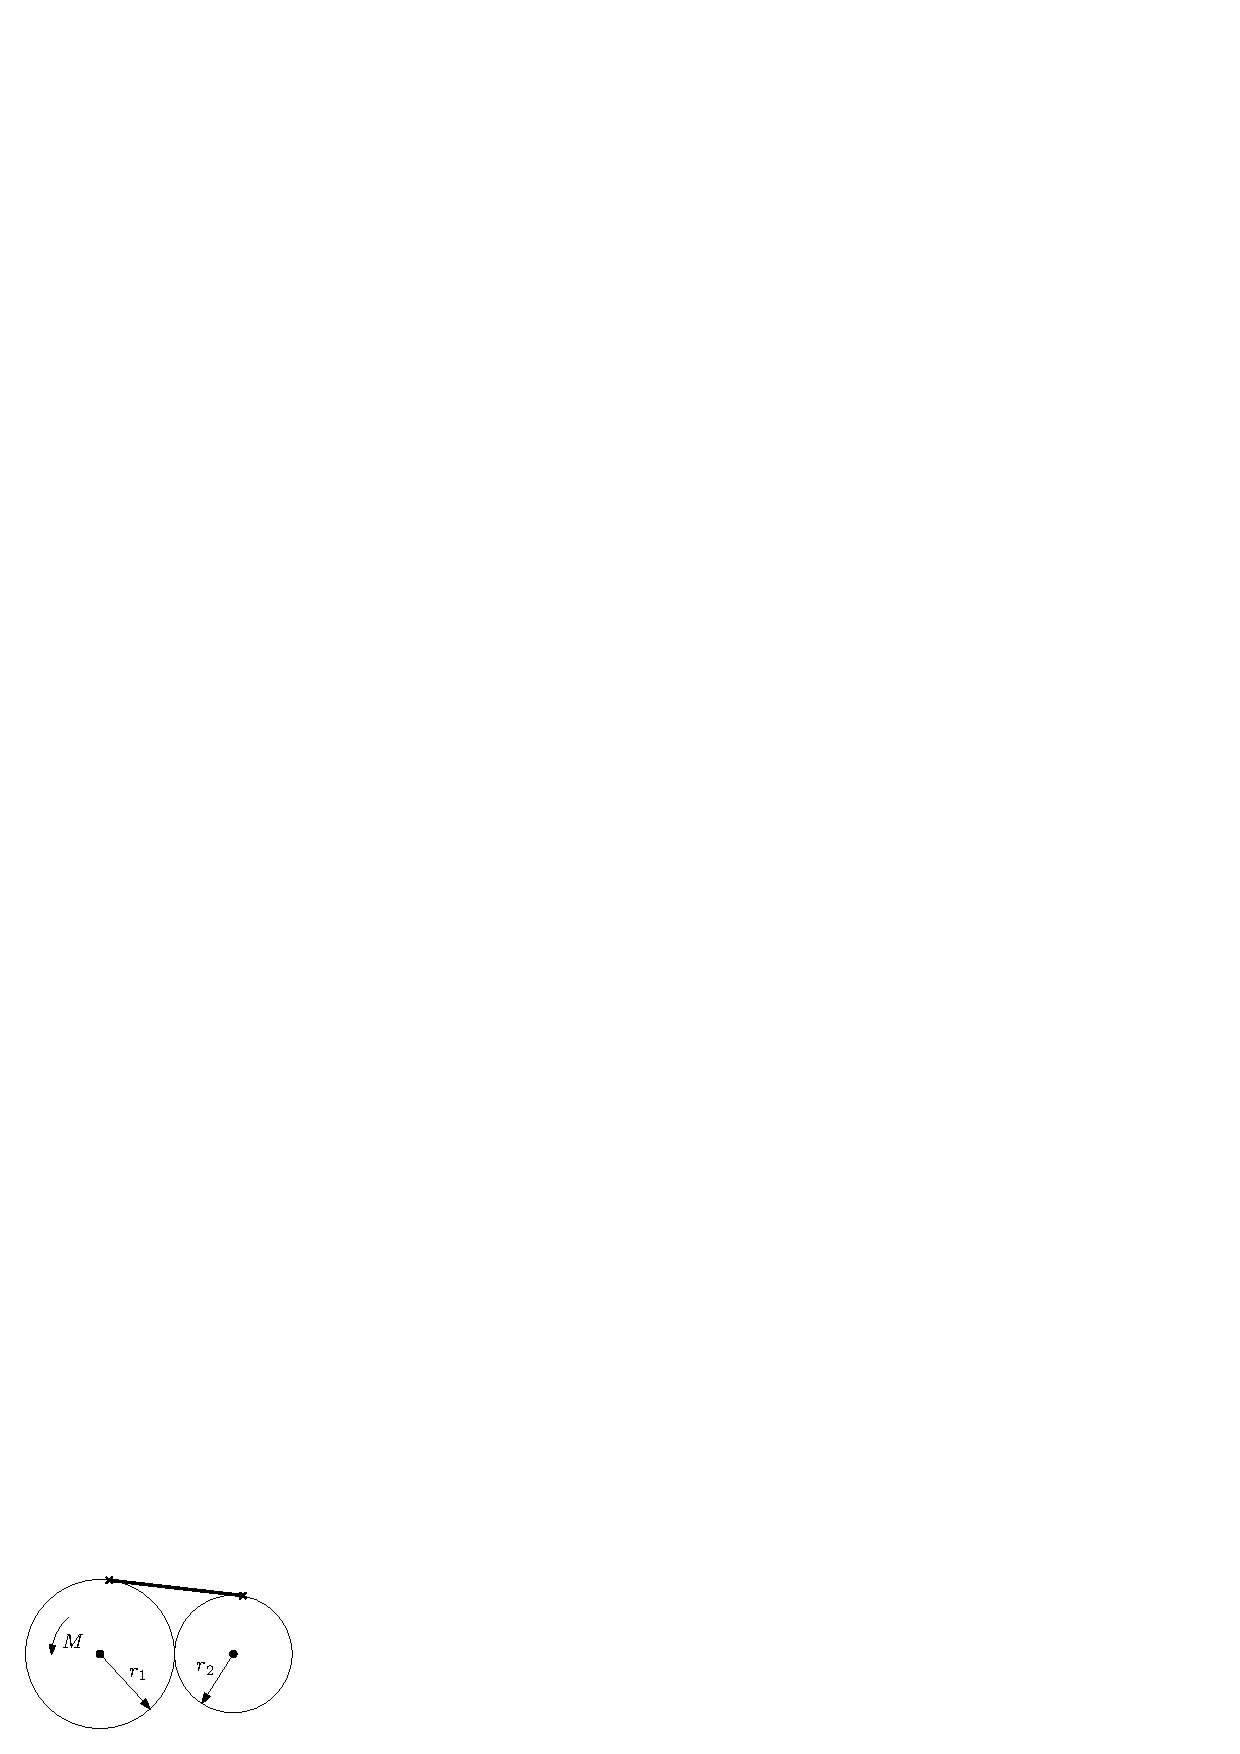
\includegraphics{2010-v3g-04-joonis_hr_ipe.pdf}
\end{center}

\hint
Kuna nöör on venimatu, on mõlemad hammasrattad paigal ja seega tasakaalus. Kehtib nii jõudude, kui ka jõumomentide tasakaal. Antud juhul on kõige mugavam vaadelda jõumomentide tasakaalu hammasrataste keskpunktide suhtes.

\solu
Kasutame virtuaalse nihke meetodit: oletame, et nöör pole siiski päris venimatu ning
saame esimest ratast pöörata väikese nurga $\alpha$ võrra. Hõõre puudub,
mistõttu salvestub kogu välise jõumomendi töö nööri elastsusjõu potentsiaalseks
energiaks. Välisjõumomendi töö on $M \alpha$ (kui jõumomenti avaldab üks jõud
õlaga $\tilde o$ ja suurusega $M / \tilde o$, siis nihkub ta rakenduspunkt $\alpha
\tilde o$ võrra ja töö on $\alpha \tilde o M / \tilde o = M \alpha$). Väikesel
nihkel ei jõua $T$ oluliselt muutuda, seega peab nööri venitamise töö olema $T
s$, kus $s$ on nööri pikenemine. Hambumusse jäävate hammasrataste pinnapunktide
läbitavad teepikkused on võrdsed --- mõlemal $\alpha r_1$, järelikult $s = 2
\alpha r_1$ ja $M \alpha = 2 \alpha r_1 T$, kust $T = \frac{M}{2 r_1}$.

\vspace{0.5\baselineskip}
\textit{Alternatiivne lahendus}\\
Ratastele mõjuvad jõud ja jõumomendid on tasakaalus. Lihtsaim on kirjutada
jõumomentide tasakaalud rataste tsentrite suhtes, kuna siis on võllide poolt
avaldatava tundmatute jõudude õlad nullid. (Muidu saame lahenduse, kui avaldame
need jõud jõudude tasakaaluvõrranditest.) Rattad mõjutavad teineteist
puutujasihilise jõuga; kui teine ratas avaldab esimesele jõudu $\vec F$, siis
avaldab Newtoni III seaduse järgi esimene teisele $-\vec F$. Jõumomentide
tasakaal esimesele rattale on nii $M = (F+T) r_1$ ning teisele $T=F$, sestap
$T = \frac{M}{2 r_1}$.
\probend